\documentclass[a4paper,11pt,twoside,openright]{scrbook}

\usepackage{swThesis}
\usepackage{amsmath}
\usepackage[htt]{hyphenat}
\usepackage{lipsum}
\usepackage{standalone}
\standalonetrue

\bibliography{bibliography}

% Figures
\graphicspath{./figs}

\begin{document}

\chapter{Cheminformatics and high-content imaging} \label{chapter:cheminformatics}

\section{Introduction}

% aim of the chapter

\subsection{Cheminformatics}
% Introduction to cheminformatics

\subsection{Structure activity relationships}
% structure activity relationship
% how chemical structures can be represented
    % SMILES, SDF

\subsection{Chemical similarity}
% chemical similarity
    % required properties of a chemical fingerprint
    % daylight fingerprints + tanimoto distances
    % ECPF? fingerprints

\subsection{Previous work in this field}
% previous attempts to map chemical structure to gene-expression?
% paper by Bender, Young et al chemical structure phenotype..

\section{Results}

% prediction un-annotated compound MOA from the annotated datasets

% compare MOA prediction from phenotypic data with the predicted target obtained
% from chemical similarity matches to public databases (ChEMBL)

% evaluation of how chemical similarity matches phenotypic similarity within the
% BioAscent dataset

\subsection{The BioAscent library contains clusters of phenotypically similar compounds}

In order to compare the phenotypic profiles produced by compounds in the BioAscent library, active compounds were selected based on on the L$_1$ norm distance from the negative control centroid (figure (\ref{figure:compound_activity})).
As many of the compounds were cytotoxic and produced images containing only a few dying cells which do not produce robust morphological measurements, an activity window was used to exclude cytoxic compounds.


\begin{figure}
    \captionsetup{width=0.8\textwidth}
    \caption[Selecting active compounds based on distance]{
Selection of active BioAscent compounds based on the L$_1$ norm distance from the DMSO negative control centroid in PCA space.
Lower and upper bounds of the selected compounds are indicated by dashed lines. In total 1244 compounds were selected.}
    \includegraphics[width=0.6\textwidth]{ch5compoundActivities}
    \label{figure:compound_activity}
\end{figure}

Hierarchical clustering of morphological profiles produced by these phenotypically active compounds showed that despite the chemical diversity of the BioAscent library, the active compounds formed distinct clusters of compounds which produced similar cellular morphologies (figure \ref{figure:morph_cluster} A).

To confirm the validity of the clustering, the hierarchical labels were compared with clusters found in an unsupervised algorithm.
The morphological profiles were embedded into lower dimensional space using the t-SNE algorithm \cite{tnse_paper} which aims to preserve local structure within the data and reveals clusters of similar points in an unsupervised approach.
When these points were coloured by the cluster labels idenfified by hierarchical clustering they appeared to match up with the tSNE embedding (figure \ref{figure:morph_cluster} B).

\begin{figure}
    \captionsetup{width=0.8\textwidth}
    \caption[Morphological clustering of the BioAscent library]{
Morphological clustering of active compounds within the BioAscent library.
    \textbf{(A)} Hierarchical clustering of the 1244 active BioAscent compounds based on a distance matrix of principal components.
    Clusters formed by cutting the produced dendrogram.
    \textbf{(B)} Unsupervised t-SNE clustering of active BioAscent compounds based on principal components of morphological features.
    Points are labels derived from the hierarchical clustering.
}
    \includegraphics[width=0.9\textwidth]{ch5phenotypicClustersBoth}
    \label{figure:morph_cluster}
\end{figure}
% maybe add some images of example morphologies produced by each cluster



\subsection{The BioAscent library is chemically diverse}
The BioAscent library is marketed as chemically diverse, yet I still wanted see to what degree this is true, and if there are clusters of chemically similar compounds such as those based around a common scaffold.
All 13,000 BioAscent compounds were converted into molecular fingerprints to produce a distance matrix between all pairs of compound fingerprints, this was then clustered using agglomative hierarchical clustering.
As could be predicted, the heatmaps and dendrograms did not reveal any large clusters of structurally similar compounds in the 13,000 compound library.
This chemical diversity continued when the compounds were filtered to only contain the phenotypically active molecules.
The use of more novel compound fingerprinting techniques such as USRCAT \cite{usercat} and autoencoded features \cite{autoencoder} did not increase the degree of clustering.

%TODO insert figure of (lack of) compound similarity clustering for both 13K and
%active

Rather than looking at large-scale clustering of many thousands of compounds with hierarchical clustering, I tried the Butina clustering method to identify small collections of structurally similar compounds.
This method does not return similarity measures, but rather groups compounds into bins of similar compounds \cite{Butina1999}.
After removing clusters which contained fewer than 3 compounds, this left 96 clusters, with the largest cluster containing 20 compounds and 58\% of the clusters containing only 3 compounds (figure \ref{figure:butina_clusters}).

\begin{figure}
    \captionsetup{width=0.8\textwidth}
    \caption[Histogram of structural cluster sizes and example of molecules within a cluster]{
        \textbf{(A)} Histogram of number of compounds within structurally similar clusters, with most clusters only containing 3 molecules.
        \textbf{(B)} An example of one of the structurally similar clusters as found with the Butina clustering algorithm. 
}
    \includegraphics[width=0.5\textwidth]{ch5butinaClusterBoth}
    \label{figure:butina_clusers}
\end{figure}



\subsection{There is little evidence that structurally similar molecules produce similar cellular morphologies}

Following the premise of SAR, structurally similar molecules are likely to share the same protein binding site, therefore activiting the same or similar signalling pathways and producing similar cellular morphologies.
I investigated to what extend structurally similar molecules in the BioAscent library produce similar cellular morphologies, and also how structurally similar are compounds which were shown to produce similar phenotypes.
Using the phenotypic clusters as defined in fig.\ref{figure:morph_cluster}, I compared the structural similarity between compounds within these phenotypic clusters compared to a null distribution of compounds picked at random.
I found that compounds within phenotypic clusters were very slightly more structurally similar than compounds picked at random (figure \ref{figure:compound_pheno_corr} A, $p=1.81\times10^{-15}$, $D=0.011$, 2-sample Kolmogorov-Smirnov test).
In addition, I approach the problem from the opposite direction and investigated the phenotypic similarity within clusters of structurally similar molecules as found with the Butina clustering algorithm, compared to the phenotypic similarity between compounds picked at random from the pooled compound list of those contained within Butina clusters.
I again found that structurally similar molecules are more likely to produce similar cellular morphologies than compounds picked at random (figure \ref{figure:compound_pheno_corr} B, $p=0.037$, $D=0.018$, 2-sample Kolmogorov-Smirnov test).

Another approach is two see how well the distance matrix of phenotypic profiles correlates with the distance matrix of chemical structures.
Using Mantel's test of correlation between two distance matrices \cite{Mantel1967}, I found no significant correlation between the phenotypic and structural distance matrices for the active 1244 compound subset ($r = 0.02$, $p = 0.116$).


\begin{figure}
    \captionsetup{width=0.8\textwidth}
    \caption[Comparison of structural and phenotypically similar compounds]{
        \textbf{(A)} Tanimoto distance between compounds from within phenotypic clusters (as found in fig. \ref{figure:morph_cluster}) and between randomly paired active compounds.
        ($p=1.81\times10^{-15}$, $D=0.011$, 2-sample Kolmogorov-Smirnov test)
    \textbf{(B)} Phenotypic distance between compounds from within structurally similar clusters and between randomly paired phenotypic profiles.
    ($p=0.037$, $D=0.018$, 2-sample Kolmogorov-Smirnov test)
}
    \includegraphics[width=1.0\textwidth]{ch5compoundSimilarity}
    \label{figure:compound_pheno_corr}
\end{figure}





\subsection{Identifying the putative MoA of phenotypic hits with ChEMBL structure queries}

Another way to utilise the chemical structure data availble with the BioAscent library is through querying publically available databases such as ChEMBL for exact compounds matches or structurally similar compounds.
This returns large amounts of data from a variety of assays in which the compound or a structural analogue was screened against such as targets, EC/IC$_{50}$ values, binding affinities etc.
I set about to see if this historical data could be used to suggest putative MoAs of hits from target agnostic phenotypic screening assays.

For this I used the compounds within 10 phenotypic clusters (figure \ref{figure:morph_cluster}), and for each cluster queried ChEMBL based on a structure similarity search to identify records for either the query compound, or structural analogues.
Then using these compounds identifying which human proteins they have been screened against, and filtering these protein based on EC/IC$_{50}$ values.
This returns a list of Uniprot accession codes which were used with interpro \cite{Finn2017} to test for enrichment compared to a background for each cluster.

Eight out of the ten phenotypic clusters returned at least one significantly enriched target with fold-enrichment ranging between 1.5 and 10.
The most significantly enriched target in 6/8 of the clusters was related to protein kinases, whereas the remaining two were rhodopsin-like GPCRS and adrenergic receptors.

\begin{figure}
    \captionsetup{width=0.8\textwidth}
    \caption[Interpro target enrichment]{
        Enriched interpro targets associated with compounds within one phenotypic cluster.
}
    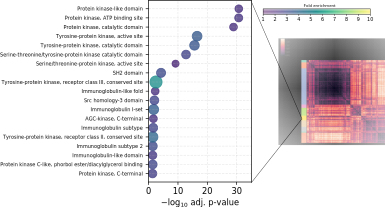
\includegraphics[width=0.8\textwidth]{ch5interpro.png}
    \label{figure:interpro}
\end{figure}



\subsection{Finding phenotypic hits to target ``dark chemical space''}

An area of interest in drug discovery is finding new pharmacologically active compounds which occupy new areas of chemical space. \cite{Wassermann2015}
One way to incoporate the phenotypically active hits from the BioAscent library is to query historical screening databases by structural similarity.
To do this I took the list of 1244 phenotypically active BioAscent compounds and performed a structural similarity search on the ChEMBL database to look for those BioAscent compounds which have a large Tanimoto distance from all compounds deposited in the database.

From the 1244 active BioAscent compounds 59 (4.7\%) were found to have no structurally similar analogues in the ChEMBL database (figure \ref{figure:dark_mols}).
To assess if these 59 compounds contained undersireable physiochemical properties which would limit their inclusion in screening libraries explain their absence from historic screening databases I used a quantitative estimate of drug-likeness (QED), \cite{Bickerton2012} to compare the 59 compounds from `dark chemical space' to the 1244 active BioAscent compounds.
The QED metric did not reveal any significant differences in desirable physiochemical properties (QED$_{\text{dark compounds}} = 0.57$,  QED$_{\text{all active}} = 0.60$, 2 sample t-test $t=0.85$, $p=0.39$).


\begin{figure}
    \captionsetup{width=1.0\textwidth}
    \caption[BioAscent hits from dark chemical space]{
BioAscent hits from dark chemical space.
59 phenotypically active BioAscent compounds which had no structurally similar compounds listed in the ChEMBL database as measured.
}
    \includegraphics[width=1.0\textwidth]{ch5darkmols}
    \label{figure:dark_mols}
\end{figure}

%TODO? map all compounds in 2D space, highlighting the dark mols, see if they
%cluster somewhere or are mixed in with all the rest


\section{Discussion and Conclusions}
TODO
% chemical similarity is difficult
% rapidly evolving field
% activity cliffs - binding properties change despite very similar structures
% bind to different targets within the same pathway - similar phenotype but can
% be very different structures


\section{Methods}

\subsection{Chemical similarity}
Compound structural information was in the form of .sdf files provided by BioAscent.
To create daylight-like compound fingerprints the RDKit library was used to convert .sdf entries into an RDKit's implementation of the daylight fingerprint using the `rdkit.Chem.Fingerprints.FingerprintMols' function with default parameters.

USRCAT features were generously calculated and supplied by Dr. Steven Shave (Edinburgh).

Latent representations of chemical structure features were calculated using a molecular autoencoder pre-trained on the ChEMBL22 dataset \footnote{www.github.com/cxhernandez/molencoder}, based on the work published by Gomez-Bombarelli \textit{et al.} \cite{Gomez-Bombarelli2016} using one-hot encoded SMILE strings of the molecules.

To compute the distance between RDKit daylight fingerprints the Tanimoto/Jaccard distance was used, in the case of USRCAT and autoencoded features I used the Euclidean distance.
Hierarchical clustering was performed on the distance matrix using the complete linkage method and euclidean distance.
To define clusters from the calculated dendrogram, a threshold was defined as 70\% of the maximum linkage distance which produced 10 clusters.
Butina clustering was implemented using RDKit with Tanimoto distances calculated from daylight fingerprints, with a cutoff value of 0.2.

Mantel's test for comparing two distance matrices was implemented with scikit-bio's implementation using Pearson's correlation coefficient and 999 permutations for testing significance.
The distance matrices used were standardised Euclidean distance for the morphological profiles and standardised Tanimoto distances of the daylight fingerprints for compound structure profiles.


\subsection{BioAscent library screen}

\subsubsection{Compound activity window}
Data was normalised to plate-based controls and features standardised, then transformed with PCA to the minimum number of principal components which accounted for 80\% of the variance in the data.
L$_1$ norm distances were calculated from the DMSO negative control centroid in PCA space.
The lower bound of the activity window was defined visually using a plot of ranked L$_1$ distances.
The upper bound was chosen based on images containing at least 10 cells and visual assessment of images produced by higher L$_1$ distances ensuring images did not consist entirely of dying cell (small, rounded and bright cytoplasmic staining).


\subsection{Phenotypic similarity}
Clustering of morphological profiles was carried out by first calculating a correlation matrix between between all pairs of active compound morphologies.
Hierarchical clustering was performed on the correlation matrix using the complete linkage method and euclidean distance.
To define clusters from the calculated dendrogram, a threshold was defined as 70\% of the maximum linkage distance which produced 10 clusters (figure \ref{figure:dendrogram_cut})

\begin{figure}
    \captionsetup{width=0.8\textwidth}
    \caption[Dendrogram threshold to determine clusters]{
Dendrogram thresholding to determine the number of phenotypic clusters in the active BioAscent compounds.
Dashed line indicates cutoff of 70\% of the maximum linkage distance, resulting in 10 clusters.
}
    \includegraphics[width=0.8\textwidth]{ch5dendrogram}
    \label{figure:dendrogram_cut}
\end{figure}

t-SNE clustering was performed using sklearn's `manifold.TSNE` implementation using the Barnes-Hut approximation with the default parameters.

\subsection{ChEMBL structure searches}
To query the ChEMBL database I used the ChEMBL webresource client \footnote{https://github.com/chembl/chembl\_webresource\_client}.
In order to identify records for similar compounds I first queried structures based on SMILE strings of the BioAscent compounds with a filter to return only compounds with a Tanimoto distance less than 0.1, recording the similar compounds as ChEMBL identifiers.
Then in a second query using the ChEMBL identifiers, I searched for historical screening results against human protein targets and returned a list in the form of Uniprot accession codes.
As this returned a list of all protein targets which had been screened against, I filtered this list to protein targets with an assay EC/IC$_{50}$ value less than 1 $\mu$M.
This was repeated for each cluster of BioAscent compounds returning a list of Uniprot accession codes for each cluster.

To search for active compounds in the BioAscent library which are structurally distinct from any compounds in the ChEMBL database I queried the ChEMBL webresource with the 1244 active BioAscent compounds, returning ChEMBL compounds wit a similarity of 70\% relating to a Tanimoto distance of the daylight fingerprints of within 0.3 (the minimum similarity value allowable with the ChEMBL API).
Any BioAscent compound that failed to return any structurally similar ChEMBL record was listed as a `dark SMILE'
\footnote{A thanks to Michał Nowotka from EMBL-EBI for making changes to the ChEMBL servers and API to allow for such time-intensive queries.}.
QED values were computed using RdKIT's Chem.QED.qed function on molecules computed from the supplied .sdf file.

\subsection{Interpro analysis}
Interpro analysis was carried out using DAVID 6.8. \cite{Huang2009}
DAVID was chosen despite more up-to-date alternatives, as DAVID allows uploading a custom background list.
Therefore I created a background list of protein targets by repeating the Uniprot lookup as before but with a list of all 12,000 BioAscent compounds, which was used as a background for each cluster.
Significantly enriched interprot targets were selected based on a Benjamini-Hochberg corrected p-value with an $\alpha$ of 0.05.



%\printbibliography

\end{document}
